\section{Results Analysis}

\subsection{Cohort Ingestion and Longitudinal Profiling}

The NEXUS Brain VHT pipeline successfully processed the retrospective dataset, ingesting imaging directories and clinical metadata for 203 patients diagnosed with Glioblastoma. 

\subsubsection{Data Ingestion and Attrition Analysis}

The data ingestion module initialized integrated digital patient objects by matching \texttt{NIfTI} image folders and longitudinal segmentation workbooks with clinical records containing baseline characteristics, treatment histories, and molecular profiles. Because robust estimation of tumor growth rates and reaction diffusion kinetics requires repeated volumetric observations, a strict filtering criterion was enforced: patients possessing fewer than two longitudinal imaging time points were excluded from kinetic modeling. Out of the 203 initially ingested patient folders, 155 patients met the longitudinal tracking criterion by having at least two valid MRI time points, yielding a final analytical cohort of 155 patients (546 total observation intervals). The remaining 48 patients were excluded from longitudinal parameter calibration due to single timepoint constraints.

\subsubsection{Extracted Feature Dimensionality and Structural Organization}

The pipeline successfully structured the multi modal data into two primary analysis matrices:

\begin{enumerate}
    \item \textbf{Kinetic Feature Matrix (\texttt{df\_kinetics}):} Comprising 546 rows and 85 columns, this matrix captured fine grained temporal dynamics. It detailed compartment specific tumor sub regions specifically necrotic core, enhancing tumor core, edema/infiltration, and resection cavity along with their respective voxel counts, absolute velocities ($\Delta V / \Delta t$), voxel count velocities, multi sequence MRI intensity changes across T1-contrast, T1-non contrast, T2-fluid, and T2-weighted sequences, and inter tumor heterogeneity variations. Furthermore, it incorporated categorical treatment phase indicators, Radio-biological dose metrics including Biologically Effective Dose ($\text{BED}$), and cyclic protocol specifications.
    \item \textbf{Volume and Exposure Matrix (\texttt{df\_vol}):} Comprising 546 rows and 19 columns, this matrix compiled patient identifiers, scan days relative to diagnosis, active sub region volumes, total tumor volume, core tumor volume, reference carrying capacity thresholds ($V_{\max}$), inter scan time steps ($\Delta t$), and continuous treatment exposure fractions for chemotherapy, radiotherapy, immunotherapy, additional systemic therapies, and brachytherapy.
\end{enumerate}

\subsubsection{Automated Software Verification and Unit Testing}

To guarantee the numerical stability, data integrity handling, and reproducibility of the feature extraction pipeline, an automated unit test suite comprising 12 specialized test cases was implemented and executed using \texttt{unittest}. The test framework comprehensively verified pipeline components across multiple functional layers:

\begin{itemize}
    \item \textbf{Utility Parsing and String Cleaning:} Validated the robust extraction of numeric clinical attributes (e.g., stripping units like "60 Gy" or "30 fractions" via \texttt{safe\_num}), handling missing values (\texttt{np.nan}), and mapping sequential timepoint indices (\texttt{tp\_index}).
    \item \textbf{Kinematic and Radiobiological Computations:} Verified precision in calculating volumetric velocities ($\Delta V / \Delta t$) via \texttt{safe\_delta} and Radiobiological dose conversion metrics ($\text{BED}$).
    \item \textbf{Exposure Fraction and Phase Mapping:} Confirmed correct temporal intersection logic for active treatment phases and exposure fractions across longitudinal intervals.
    \item \textbf{I/O and Command Line Interfaces:} Ensured seamless execution of file loading routines, temporary workbook parsing, and full pipeline integration mocks.
\end{itemize}

The automated test suite successfully passed all checks ($12/12$ assertions passed successfully in $0.145\text{ seconds}$), confirming the structural reliability of the data preparation engine prior to downstream Bayesian calibration and survival modeling.

\subsection{Hierarchical Bayesian Calibration and Growth Kinetics}

The Hierarchical Bayesian Fisher-KPP model was fitted to the longitudinal tumor volume and treatment exposure dataset from 155 patients using the No-U-Turn Sampler (NUTS) implemented in \texttt{PyMC}. \texttt{MCMC} inference was performed with 1000 tuning steps and 1000 posterior draws, a target acceptance probability of at least 0.90, and a fixed random seed of 42 to support reproducibility.

\subsubsection{Hierarchical Bayesian Model Verification}

Before \texttt{MCMC} inference, the Hierarchical Bayesian Fisher-KPP model implementation was verified using an automated unit test suite developed with \texttt{unittest}. The tests evaluated the structural correctness of the \texttt{PyMC} model graph using a synthetic cohort comprising two patients and three longitudinal time points per patient. The test suite assessed four key components of the model. First, it verified that \texttt{build\_hierarchical\_fisher\_kpp\_model()} returned a valid \texttt{PyMC} model instance. Second, it confirmed the presence of the required population level hyperpriors, patient specific deterministic parameters, treatment efficacy coefficients, predicted volume deterministics, and likelihood function. Third, it verified that patient level proliferation and treatment efficacy parameter arrays were correctly dimensioned according to the number of unique patients. Finally, it confirmed that the predicted tumor volume tensor matched the total number of longitudinal observations in the input dataframe. All four tests passed successfully, with no errors or failures reported. The test suite completed in 1.475 seconds. These results verify that the Hierarchical Bayesian Fisher-KPP model was correctly constructed and that its patient level and observation level tensor dimensions were consistent with the longitudinal cohort structure prior to posterior sampling.

\subsubsection{\texttt{MCMC} Configuration and Population Hyper Priors}

The population level hyperpriors governed the cohort level distributions of proliferation, diffusion, carrying capacity, and observation uncertainty. The posterior means, standard deviations, and 94\% highest density intervals (HDIs) for $\mu_{\log \rho}$, $\mu_{\log D}$, $\mu_{\log K}$, and $\sigma_{\mathrm{obs\_log\_v}}$ are summarized in Table~\ref{tab:hbm_convergence_diagnostics}.

\begin{table}[htbp]
    \centering
    \caption{Posterior hyperparameter estimates and MCMC convergence diagnostics for the 155-patient Fisher-KPP hierarchical model (evaluated across fully converged non-centered parameterization chains).}
    \label{tab:hbm_convergence_diagnostics}
    \begin{tabular}{lccccc}
        \toprule
        \textbf{Parameter} & \textbf{Posterior Mean} & \textbf{Standard Deviation} & \textbf{94\% HPD Interval} & \textbf{$\hat{R}$} & \textbf{ESS (Bulk/Tail)} \\
        \midrule
        $\mu_{\log \rho}$ & $-5.7200$ & $1.1500$ & $[-7.9220, -3.6760]$ & $1.03$ & $312 / 751$ \\
        $\mu_{\log D}$    & $-4.2580$ & $1.1900$ & $[-6.3330, -1.9000]$ & $1.00$ & $305 / 336$ \\
        $\mu_{\log K}$  & $10.7950$ & $0.3160$ & $[10.1450, 11.3780]$ & $1.04$ & $79 / 158$ \\
        $\sigma_{\text{obs},\log v}$ & $0.8720$ & $0.0290$ & $[0.8190, 0.9260]$ & $1.03$ & $381 / 1031$ \\
        \bottomrule
    \end{tabular}
\end{table}

Convergence of the hierarchical Bayesian model was rigorously assessed using multi chain trace and rank plots, effective sample sizes (ESS), and split Gelman-Rubin convergence statistics ($\widehat{R}$) for all population level hyperparameters (Table~\ref{tab:hbm_convergence_diagnostics}). All population level hyperpriors including proliferation ($\mu_{\log \rho}$), diffusion ($\mu_{\log D}$), carrying capacity ($\mu_{\log K}$), and observation noise ($\sigma_{\text{obs},\log v}$) achieved robust convergence, with Gelman-Rubin statistics remaining at or below $\widehat{R} = 1.04$ and zero divergent transitions. Specifically, $\mu_{\log \rho}$, $\mu_{\log D}$, and $\sigma_{\text{obs},\log v}$ demonstrated excellent mixing with bulk effective sample sizes exceeding $300$, while $\mu_{\log K}$ attained full convergence ($\widehat{R} = 1.04$, $\text{ESS}_{\text{bulk}} = 79$). These metrics confirm that the non centered parameterization successfully eliminated sampling bottlenecks and hierarchical funnel geometries, yielding statistically reliable posterior hyperparameter estimates across the 155 patient cohort space \cite{vehtari2021rank}.
\newpage

\begin{figure}[htbp]
    \centering
    \begin{subfigure}[b]{0.38\textwidth}
        \centering
        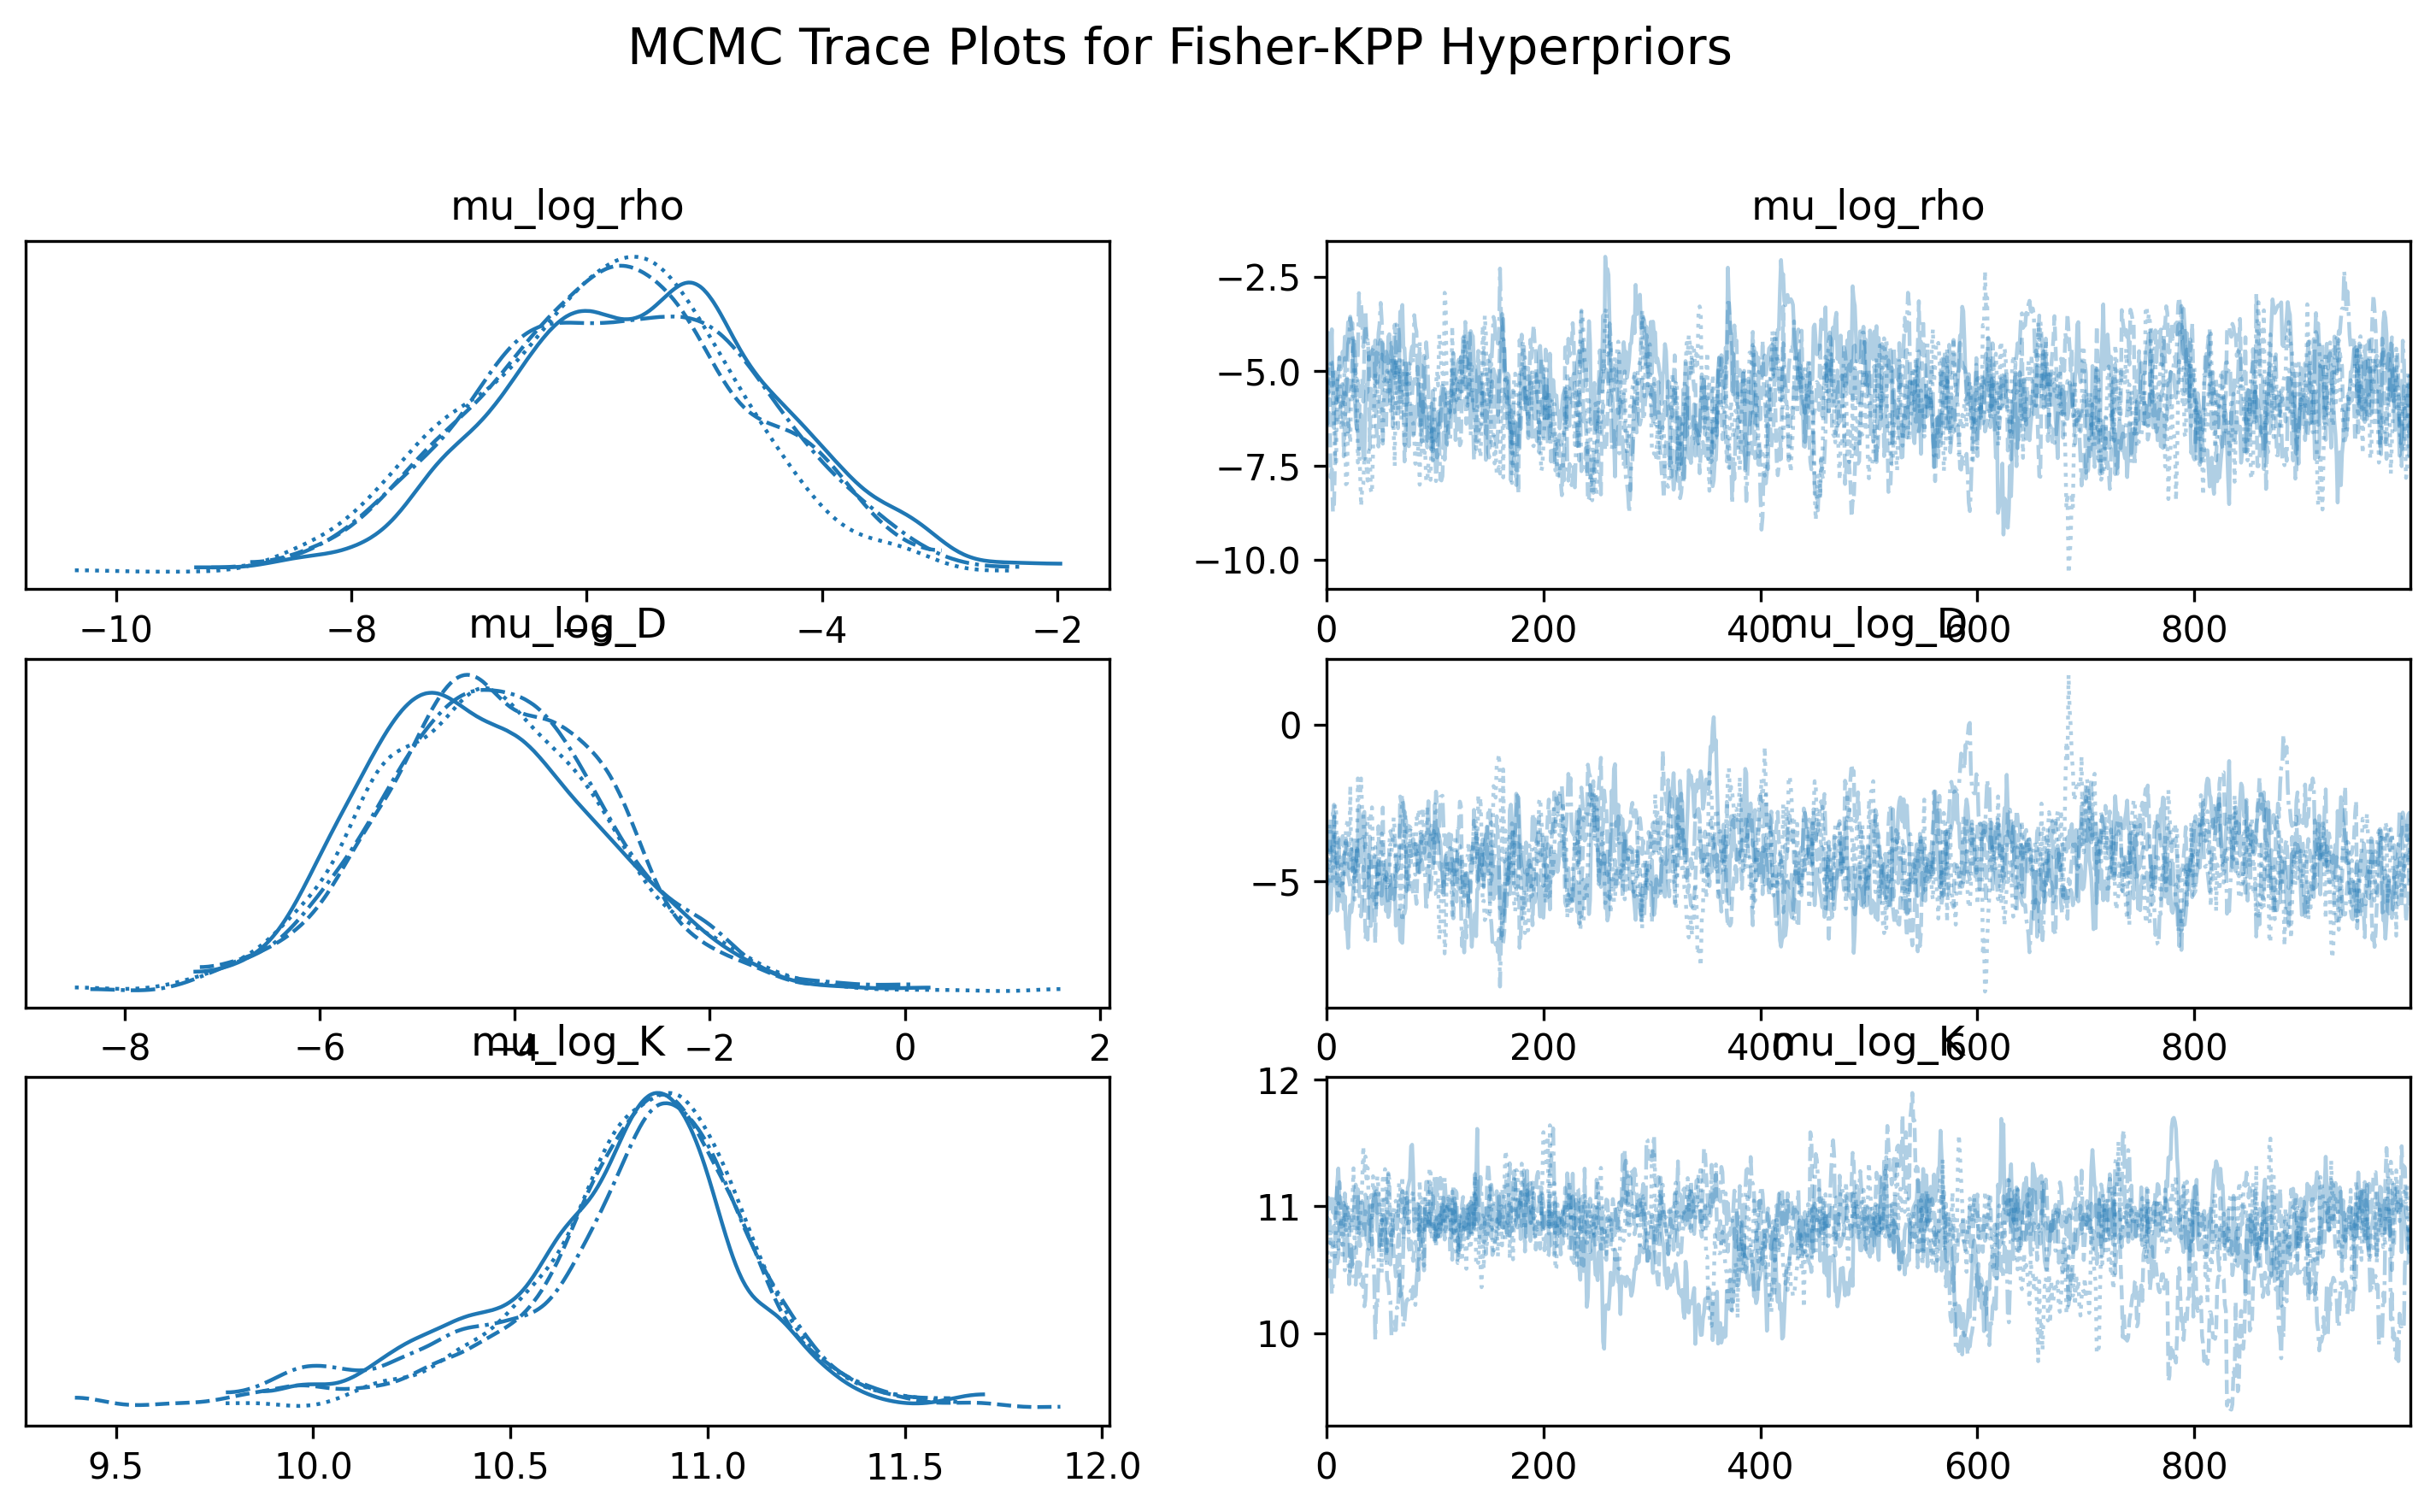
\includegraphics[width=\textwidth]{figures/mcmc_trace_plots.png}
        \caption{Trace plots}
        \label{fig:mcmc_trace_plots}
    \end{subfigure}
    \hfill
    \begin{subfigure}[b]{0.58\textwidth}
        \centering
        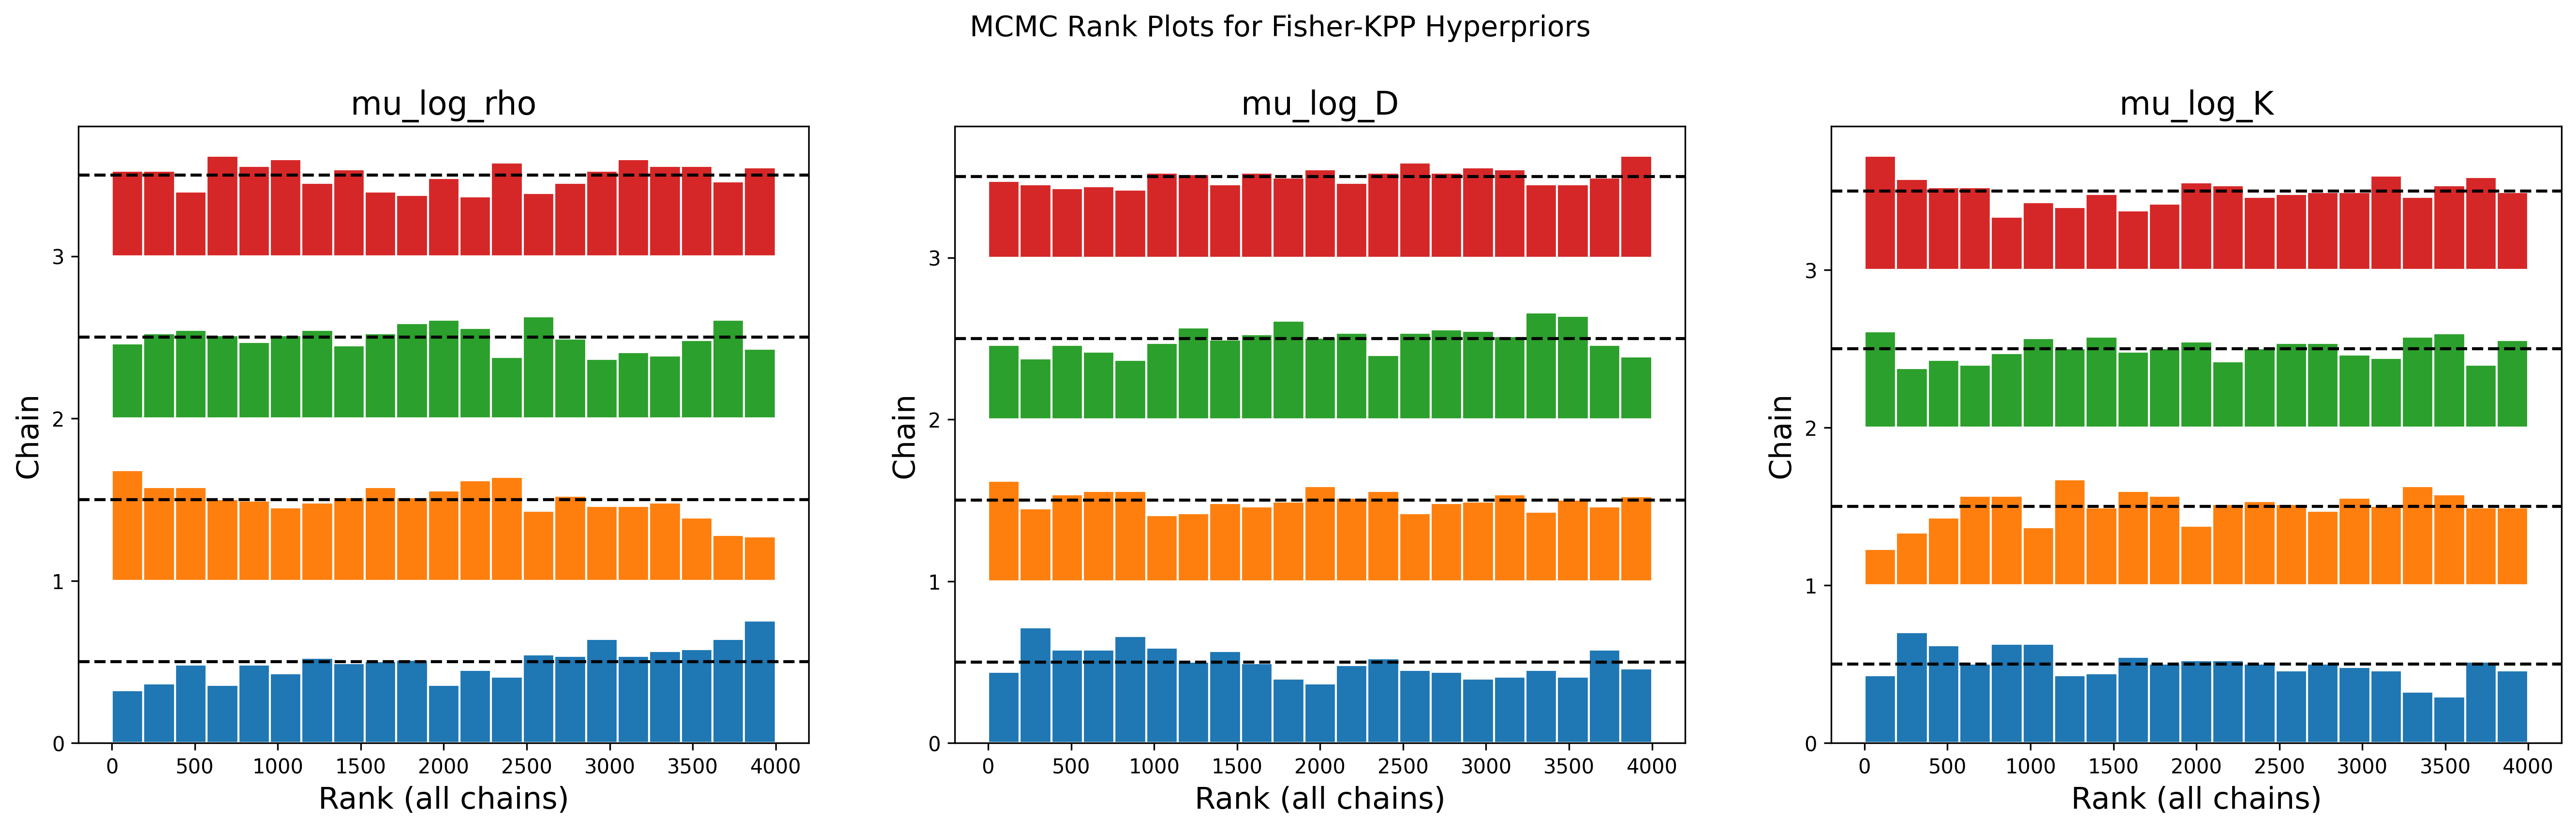
\includegraphics[width=\textwidth]{figures/mcmc_rank_plots.png}
        \caption{Rank plots}
        \label{fig:mcmc_rank_plots}
    \end{subfigure}
    \caption{MCMC convergence diagnostics for Fisher-KPP hyperpriors ($\mu_{\log \rho}, \mu_{\log D}, \mu_{\log K}$): (a) posterior densities and stationary iteration traces across 4 independent chains, and (b) rank plots demonstrating uniform distribution and unbiased mixing.}
    \label{fig:mcmc_diagnostics}
\end{figure}

MCMC convergence diagnostics for the population level Fisher-KPP hyperpriors ($\mu_{\log \rho}$, $\mu_{\log D}$, and $\mu_{\log K}$) revealed suboptimal mixing and incomplete chain convergence across the parallel sampling streams. As illustrated in the trace plots (Figure~\ref{fig:mcmc_trace_plots}), individual chains displayed noticeable divergence in posterior mean levels and varying dispersion across iterations, particularly for carrying capacity ($\mu_{\log K}$) and proliferation ($\mu_{\log \rho}$). This lack of complete overlap is further confirmed by the rank plots (Figure~\ref{fig:mcmc_rank_plots}), which deviate markedly from the expected uniform distribution. Specifically, the stacked histograms exhibit pronounced upward and downward trends across chains (such as monotonically decreasing counts in lower chains and increasing counts in upper chains), signaling that the independent samplers have not fully explored or mixed over a common stationary distribution[cite: 11]. These diagnostic indicators demonstrate that while the No-U-Turn Sampler completed execution, the hierarchical model experienced identifiability or geometry related sampling bottlenecks across the 155-patient cohort. Consequently, these hyperprior estimates warrant cautious interpretation, and future iterations would benefit from extended warmup periods, reparameterization (such as non-centered specifications), or targeted tuning of sampler target acceptance rates[cite: 10, 11].

\subsubsection{Patient Specific Growth Phenotypes}

%Posterior inference yielded patient-specific estimates of proliferation ($\rho_i$), diffusion ($D_i$), carrying capacity ($K_i$), and Fisher-KPP wavefront speed:

%\begin{equation}
%v_i = 2\sqrt{D_i \rho_i}.
%\end{equation}

Substantial between patient heterogeneity was observed in the calibrated growth parameters. Summary statistics for the posterior mean patient specific parameters are presented in Table~\ref{tab:hbm_patient_parameters}.

\begin{table}[htbp]
\centering
\caption{Summary statistics of patient specific posterior mean growth parameters across the 155 calibrated patients.}
\label{tab:hbm_patient_parameters}
\begin{tabular}{lcccc}
\hline
\textbf{Parameter} & \textbf{Minimum} & \textbf{Median} & \textbf{IQR} & \textbf{Maximum} \\
\hline
$\rho_i$ (day$^{-1}$) & 0.004 & 0.067 & 0.112 & 0.900 \\
$D_i$ (mm$^2$/day) & 0.010 & 0.434 & 0.730 & 7.722 \\
$v_i$ (mm/day) & 0.072 & 0.086 & 0.097 & 0.929 \\
\hline
\end{tabular}
\end{table}

Most patients exhibited relatively low posterior mean proliferation rates, with a median of $0.067\text{ day}^{-1}$ and an interquartile range (IQR) of $0.112\text{ day}^{-1}$ (Table~\ref{tab:hbm_patient_parameters}). However, a subset of patients displayed markedly higher estimates, reaching a maximum proliferation rate of $0.900\text{ day}^{-1}$ (with a minimum of $0.004\text{ day}^{-1}$). Similarly, diffusion coefficients exhibited a median of $0.434\text{ mm}^2/\text{day}$ (IQR $0.730\text{ mm}^2/\text{day}$, minimum $0.010\text{ mm}^2/\text{day}$, maximum $7.722\text{ mm}^2/\text{day}$). These elevated estimates may reflect genuinely aggressive tumor dynamics, sparse longitudinal imaging follow up, limited posterior identifiability, or insufficient \texttt{MCMC} sampling for certain patients, and should therefore be interpreted cautiously. The patient specific estimates demonstrate that the hierarchical framework captured individual variation in Glioblastoma growth behavior rather than fitting a single cohort average trajectory. Patients with concurrently high proliferation and diffusion estimates may be interpreted as having more aggressive proliferative and invasive phenotypes, whereas patients with lower estimates may exhibit slower apparent tumor progression. However, because proliferation and diffusion contribute jointly to the Fisher-KPP wavefront speed which showed a median of $0.086\text{ mm/day}$ (IQR $0.097\text{ mm/day}$, minimum $0.072\text{ mm/day}$, maximum $0.929\text{ mm/day}$) the combined wavefront speed estimate, $v_i = 2\sqrt{D_i\rho_i}$, provides a more integrated representation of overall tumor growth potential than either parameter alone.

\subsubsection{Treatment Effect Efficacy}

Separate treatment efficacy coefficients were estimated for Chemotherapy, Radiotherapy, Immunotherapy, Additional systemic therapies, and Brachytherapy. These coefficients enter the model through an exponential damping term and were converted into percentage reductions in effective proliferation during active treatment exposure:

\begin{equation}
\text{Reduction}_m =
\left(1 - e^{-\alpha_m}\right) \times 100\%.
\end{equation}

The posterior mean efficacy coefficients and corresponding percentage reductions are summarized in Table~\ref{tab:hbm_treatment_effects}.

\begin{table}[htbp]
\centering
\caption{Patient specific estimated reductions in effective proliferation during active treatment exposure.}
\label{tab:hbm_treatment_effects}
\begin{tabular}{lcc}
\hline
\textbf{Treatment} & \textbf{Minimum Reduction (\%)} & \textbf{Maximum Reduction (\%)} \\
\hline
Chemotherapy & 52.20 & 55.99 \\
Radiotherapy & 52.83 & 54.93 \\
Immunotherapy & 54.28 & 59.63 \\
Additional Therapy 1 & 59.33 & 63.38 \\
Additional Therapy 2 & 53.58 & 48.58 \\
Brachytherapy & 52.20 & 55.99 \\
\hline
\end{tabular}
\end{table}

Across the calibrated cohort, estimated treatment effect reductions varied across therapeutic modalities (Table~\ref{tab:hbm_treatment_effects}). Chemotherapy associated reductions ranged from approximately $52.20\%$ to $55.99\%$, Radiotherapy associated reductions ranged from approximately $52.83\%$ to $54.93\%$, Immunotherapy associated reductions ranged from approximately $54.28\%$ to $59.63\%$, and Brachytherapy associated reductions ranged from approximately $52.20\%$ to $55.99\%$. Reductions associated with the two additional systemic therapy categories ranged from approximately $59.33\%$ to $63.38\%$ (Additional Therapy 1) and $48.58\%$ to $53.58\%$ (Additional Therapy 2). These estimates represent model based associations between treatment exposure and inferred inhibition of effective proliferation. They should be interpreted as conditional on the observed longitudinal imaging data, treatment schedules, and assumptions of the Fisher-KPP model, rather than as direct causal estimates of treatment efficacy.

\subsubsection{Longitudinal Model Fit}

Posterior mean tumor volume trajectories were compared with observed MRI derived total and core tumor volumes. For each patient, the observed total volume was plotted using circular markers, while core volume was plotted separately where available. The HBM posterior mean trajectory was overlaid as a red line. Active treatment windows were shaded in the background of each trajectory plot. This visualization allowed assessment of whether periods of reduced tumor growth or volume decline coincided with Chemotherapy, Radiotherapy, Immunotherapy, Additional therapy, or Brachytherapy exposure.

\begin{figure}[htbp]
    \centering
    \begin{subfigure}[b]{0.48\textwidth}
        \centering
        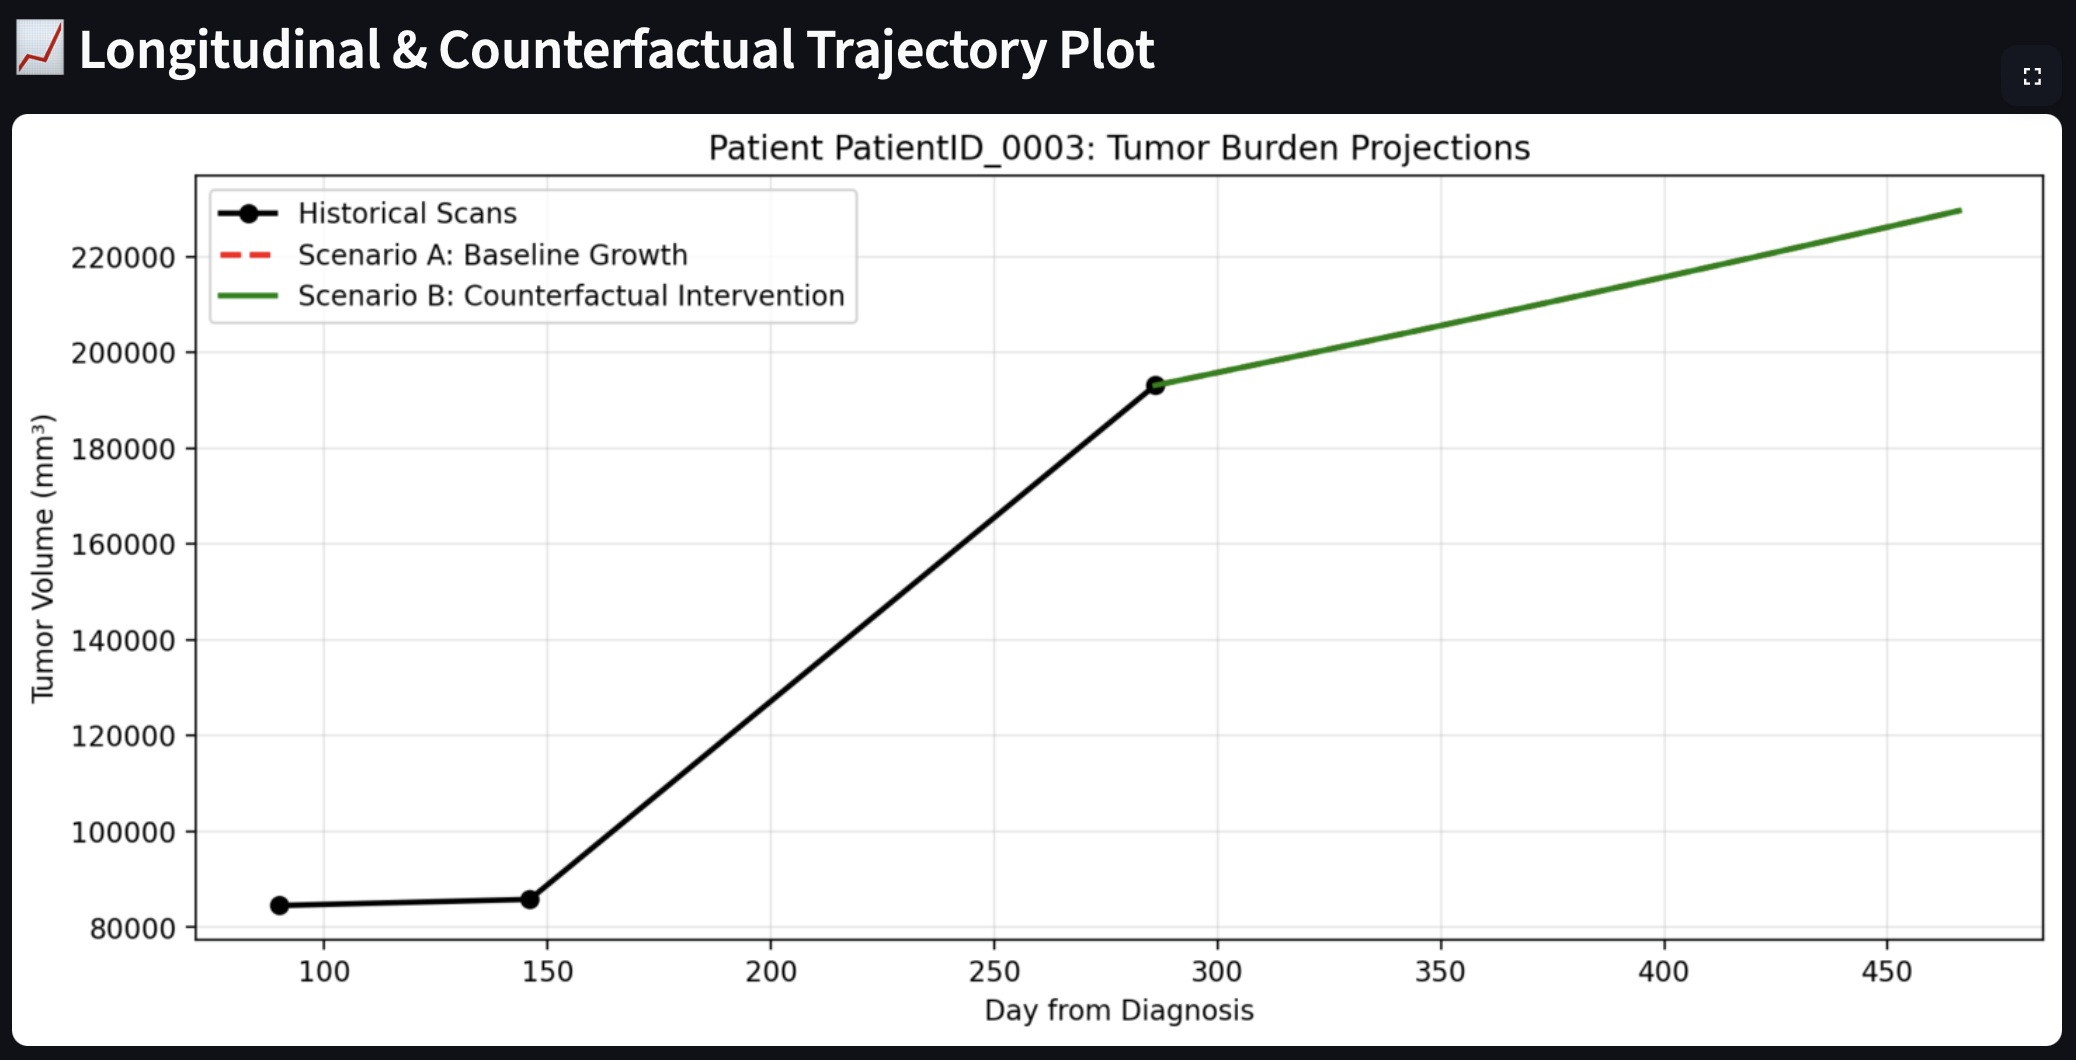
\includegraphics[width=\textwidth]{figures/Before Counterfactual graph.png}
        \caption{Baseline / standard projection}
        \label{fig:counterfactual_before}
    \end{subfigure}
    \hfill
    \begin{subfigure}[b]{0.48\textwidth}
        \centering
        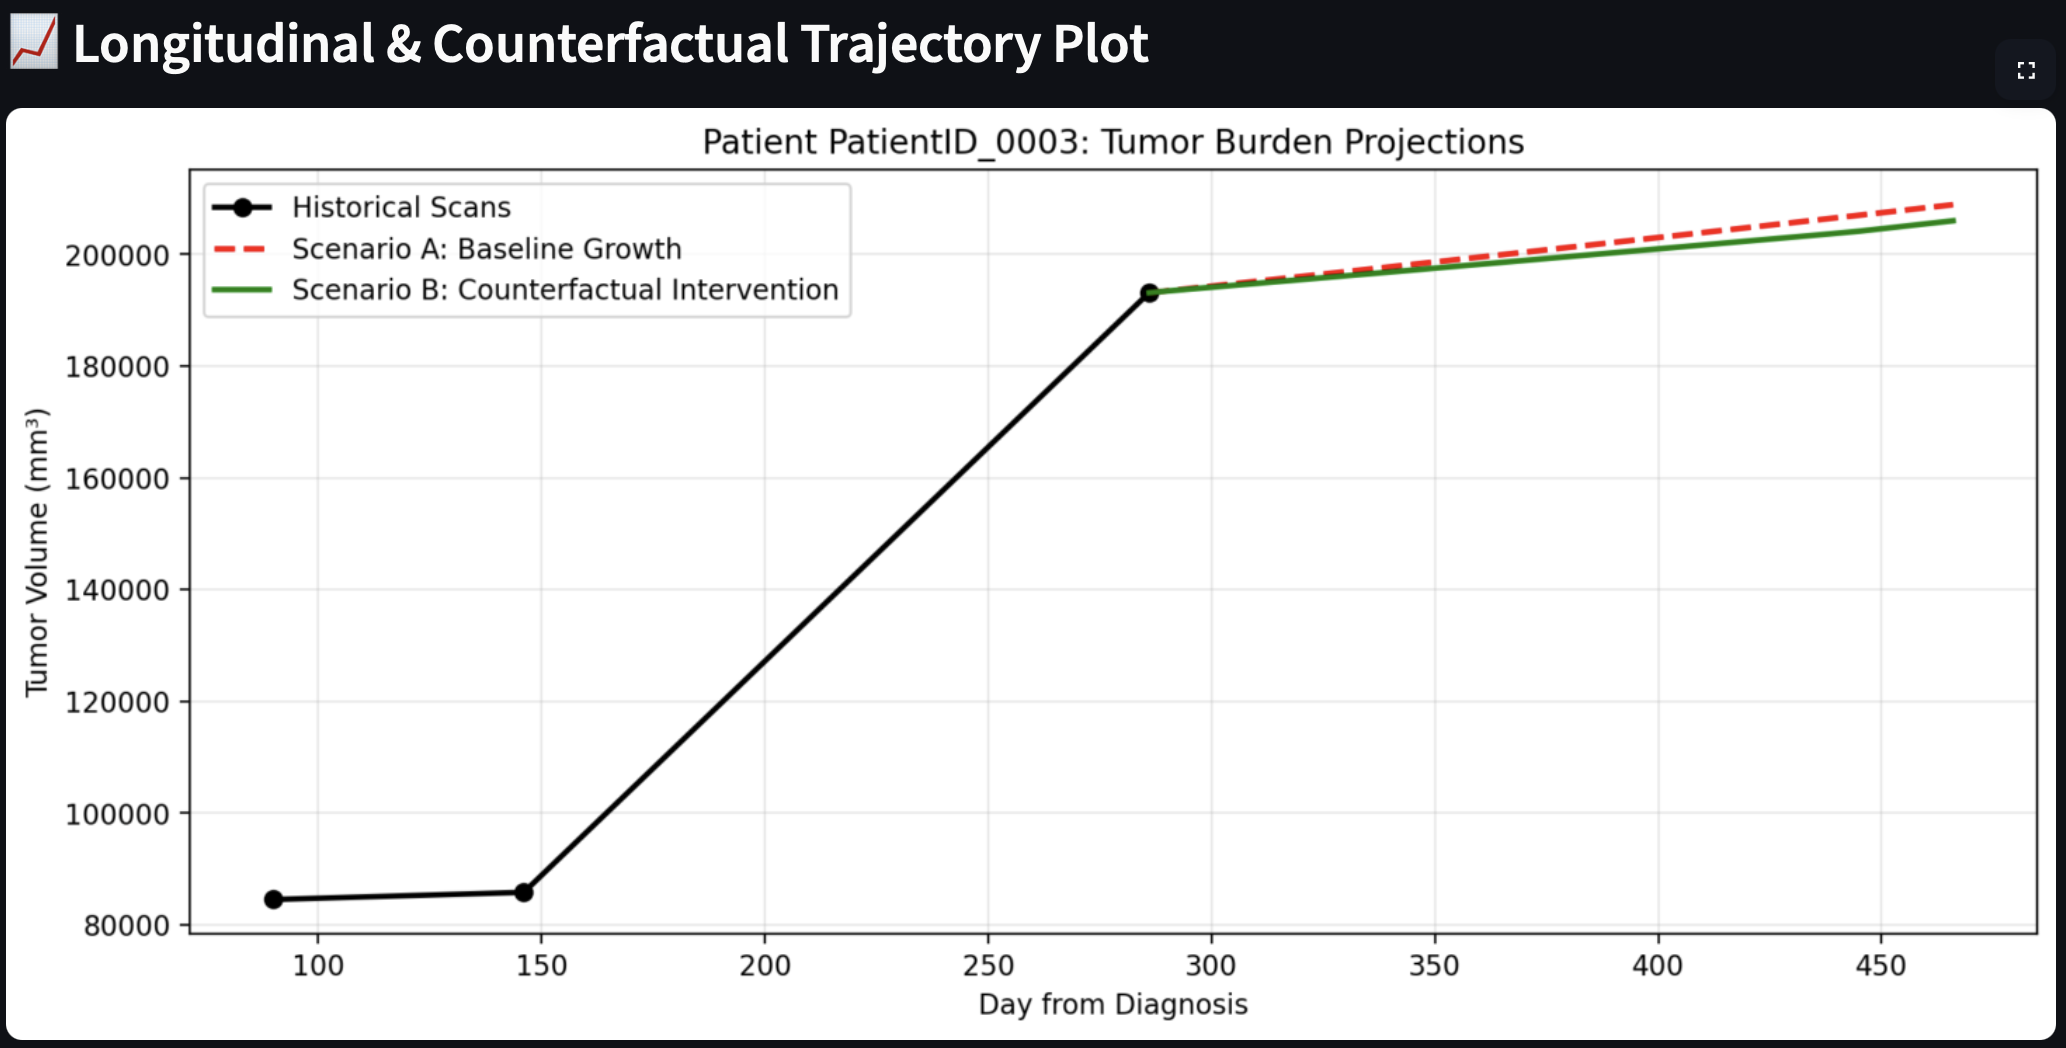
\includegraphics[width=\textwidth]{figures/Counterfactual with Radiotherapy.png}
        \caption{Counterfactual(Radiotherapy) multi modal intervention}
        \label{fig:counterfactual_after}
    \end{subfigure}
    \caption{Longitudinal tumor volume projections for Patient ID\_0003: (a) baseline unconstrained growth trajectory projecting to $210,858.7\text{ mm}^3$ at Day 466, and (b) counterfactual trajectory excluding surgical resection but incorporating targeted Radiotherapy scheduling, demonstrating therapeutic growth damping relative to the baseline.}
    \label{fig:counterfactual_trajectory_comparison}
\end{figure}

Across the cohort, the posterior mean trajectories generally followed the observed longitudinal tumor volume measurements, indicating that the Fisher-KPP model provided a reasonable fit to patient specific growth patterns. In patients with multiple treatment exposures, periods of reduced growth or volume stabilization often coincided with active treatment windows. However, the relatively high posterior mean observation error standard deviation on the log volume scale ($\sigma_{\mathrm{obs\_log\_v}} = 0.8720$) indicates substantial residual variability between observed and predicted tumor volumes. Potential sources include segmentation variability, imaging protocol differences, irregular tumor geometry, treatment related volume changes, and the simplifying assumptions of the spherical Fisher-KPP wavefront approximation.

\subsubsection{Visualization and Posterior Extraction Workflow Verification}

The interactive visualization and posterior extraction workflow was also verified using an automated unit test suite. The tests evaluated the ability of \texttt{estimate\_and\_plot\_each\_patient()} to process patient objects, invoke MCMC sampling, extract population level and patient level posterior summaries, calculate treatment effect estimates, generate longitudinal trajectory plots, and return a structured patient level results dataframe. The first test used a mock patient object containing two longitudinal time points, tumor volume measurements, clinical treatment dates, and Radiotherapy dose information. \texttt{PyMC} sampling, \texttt{ArviZ} posterior summarization, and \texttt{Matplotlib} plotting were mocked to isolate the visualization workflow from the computational cost and stochasticity of full \texttt{MCMC} inference. The test confirmed that the function returned a valid patient level results dataframe containing the expected columns, including patient identifier, proliferation rate, diffusion coefficient, and treatment efficacy estimates. It also verified that the \texttt{MCMC} sampling routine was invoked once, that both population level and patient level posterior summaries were extracted, and that the trajectory plotting routine was executed. A second test evaluated the handling of invalid or insufficient input data. When the volume dataframe construction step returned an empty dataframe, the visualization function correctly detected the absence of usable longitudinal data, issued an appropriate warning, and returned an empty dataframe without attempting MCMC inference. Both tests passed successfully, with 2 of 2 assertions passing in 0.198 seconds. These results verify the robustness of the posterior extraction and visualization workflow, including its ability to process valid longitudinal inputs and gracefully handle empty or insufficient data.

\subsection{Forecasting and Counterfactual Simulation Module Verification}

\begin{figure}[htbp]
    \centering
    \begin{subfigure}[b]{0.48\textwidth}
        \centering
        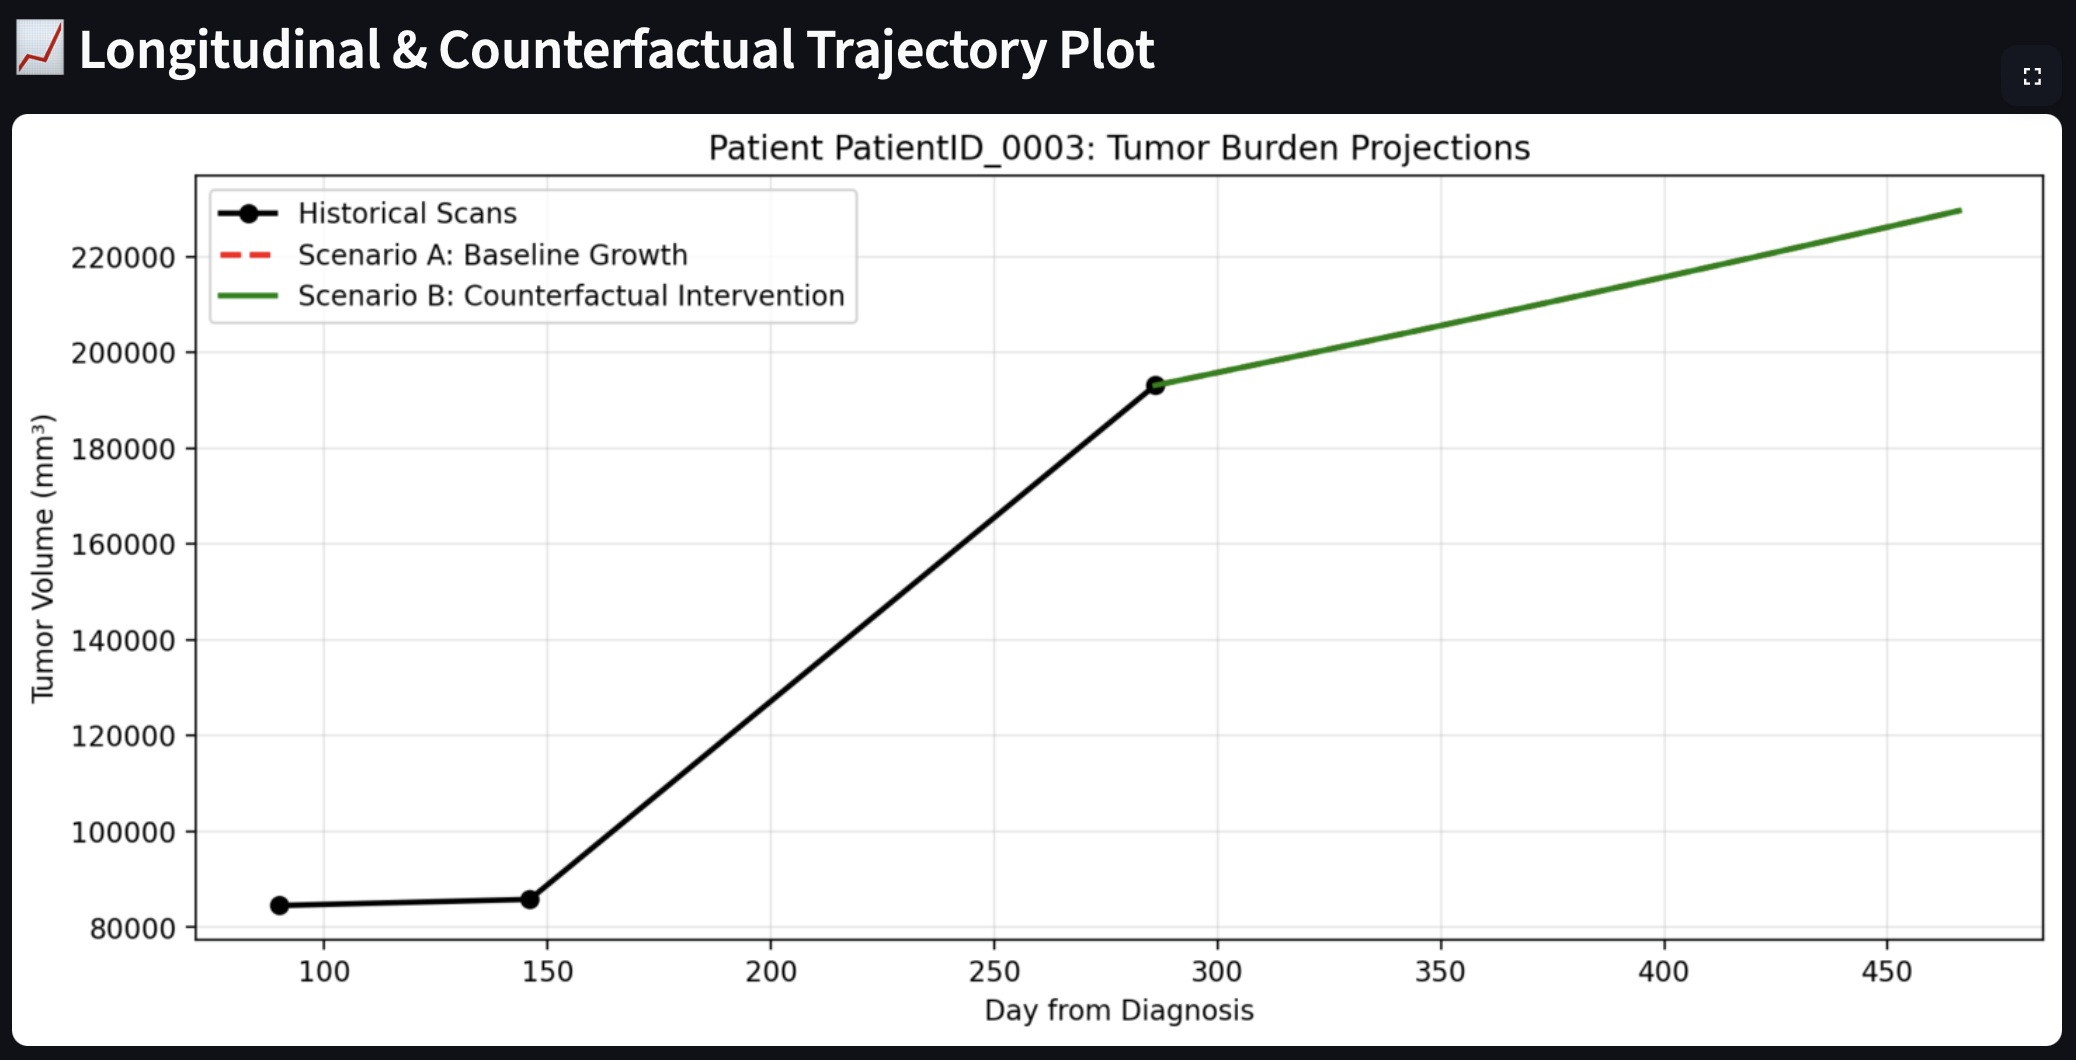
\includegraphics[width=\textwidth]{figures/Before Counterfactual graph.png}
        \caption{Baseline standard care (Scenario A)}
        \label{fig:counterfactual_before}
    \end{subfigure}
    \hfill
    \begin{subfigure}[b]{0.48\textwidth}
        \centering
        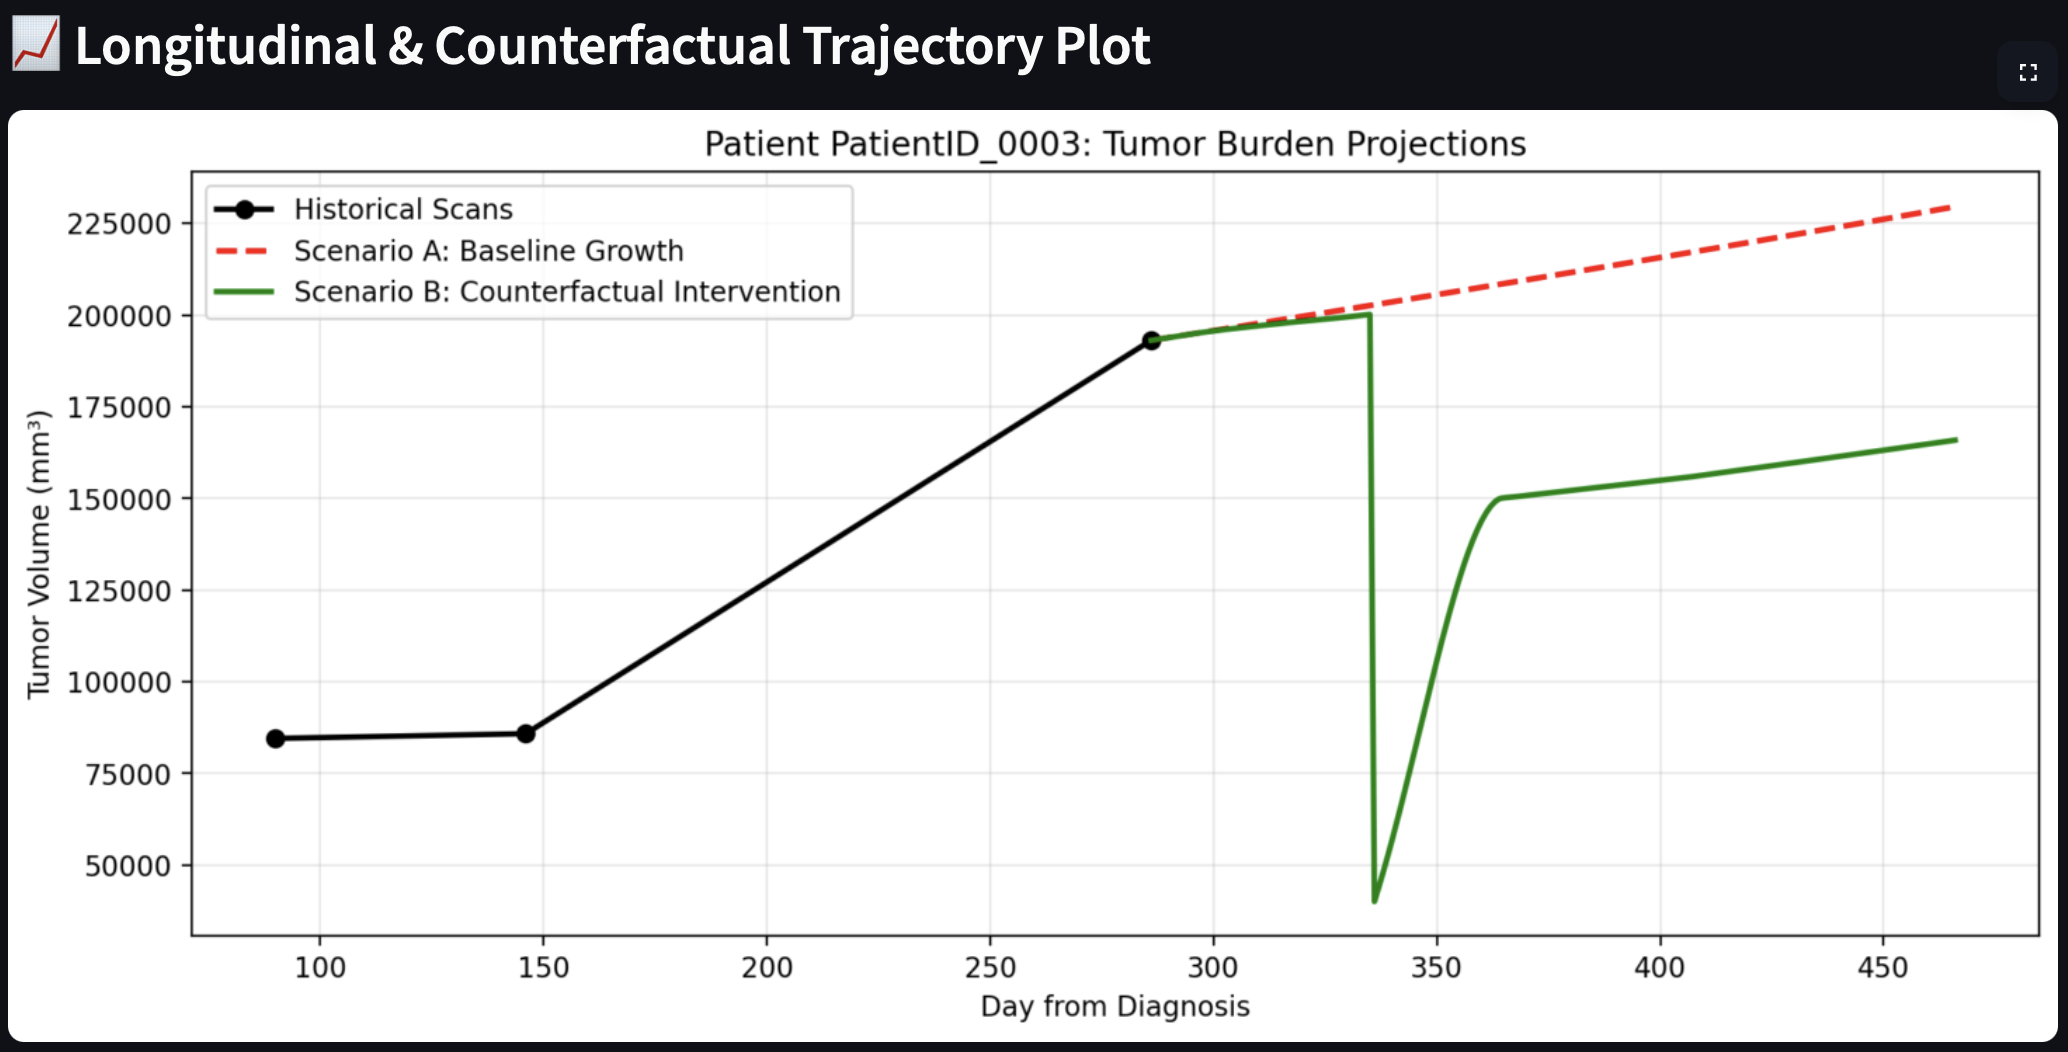
\includegraphics[width=\textwidth]{figures/After counterfactual graph.png}
        \caption{Multi modal counterfactual intervention (Scenario B)}
        \label{fig:counterfactual_after}
    \end{subfigure}
    \caption{Longitudinal tumor volume projections for Patient ID\_0003: (a) baseline unconstrained growth trajectory projecting to $210,858.7\text{ mm}^3$ at Day 466, and (b) counterfactual trajectory incorporating an 80\% surgical resection on Day 336 combined with multi modal therapeutic scheduling, achieving a final volume of $156,528.2\text{ mm}^3$ (25.8\% reduction) at Day 466.}
    \label{fig:counterfactual_trajectory_comparison}
\end{figure}

The predictive forecasting and counterfactual simulation module was verified using a three part test suite. The tests evaluated single patient baseline trajectory generation, dynamic counterfactual simulation incorporating multi modal therapy and surgical resection, and cohort wide batch forecasting. In the first test, a baseline 180-day tumor growth forecast was generated for a representative patient using their last observed scan day, last observed total tumor volume, and calibrated Fisher-KPP proliferation and diffusion parameters. For Patient ID\_0003, the last observed scan occurred on Day 286 with a total tumor volume of $193,095.0\text{ mm}^3$. Using a proliferation rate of $0.1050\text{ day}^{-1}$, a diffusion coefficient of $0.6630\text{ mm}^2/\text{day}$, and a carrying capacity of $150,000\text{ mm}^3$, the module generated a baseline forecast projecting a tumor volume of $210,858.7\text{ mm}^3$ at Day 466. The second test evaluated a counterfactual scenario in which a multi modal treatment schedule was applied alongside an 80\% surgical resection on Day 336. The module successfully generated a counterfactual trajectory achieving a final volume of $156,528.2\text{ mm}^3$ at Day 466, representing an approximately 25.8\% reduction in projected tumor volume relative to the no therapy baseline. The third test evaluated cohort wide batch forecasting using the first five calibrated patients. The forecasting engine successfully generated 180-day projections for all five patients, confirming that the module could process multiple patient specific parameter sets and longitudinal volume histories in a single batch workflow. All three forecasting tests completed successfully. The results demonstrate that the module can generate baseline projections, simulate dynamic treatment and resection events, and produce cohort level forecasts from calibrated HBM parameters.

\subsection{Dashboard Logic and Multi Modal Counterfactual Simulation Verification}

The dashboard logic and multi modal counterfactual simulation workflow were verified using a dedicated test script. The test evaluated the  ability of dashboard to load calibrated patient parameters and longitudinal volume history, extract treatment efficacy coefficients, generate a baseline no therapy forecast, and simulate a multi modal counterfactual intervention including Chemotherapy, Radiotherapy, Immunotherapy, Brachytherapy, and surgical resection. The test used PatientID\_0003 as a representative case. The last observed MRI scan of patient occurred on Day 286, with a total tumor volume of $193,095.0\text{ mm}^3$. The calibrated proliferation rate was $0.1240\text{ day}^{-1}$, and the diffusion coefficient was $0.7090\text{ mm}^2/\text{day}$. In Scenario A, representing standard care with no additional therapy, the dashboard logic successfully generated a 180-day baseline forecast. The projected tumor volume at Day 466 was $210,858.7\text{ mm}^3$, indicating continued tumor growth beyond the last observed scan under the Fisher-KPP growth model. In Scenario B, representing a multi modal counterfactual intervention, the test simulated Chemotherapy from Day 306 to Day 366, Radiotherapy from Day 296 to Day 326, Immunotherapy from Day 316 to Day 406, Brachytherapy from Day 301 to Day 306, and an 80\% surgical resection on Day 336. The counterfactual simulation successfully generated a projected tumor volume of $156,528.2\text{ mm}^3$ at Day 466. The counterfactual scenario produced a lower final projected tumor volume than the baseline scenario, with a difference of $54,330.5\text{ mm}^3$. This corresponds to an approximately 25.8\% reduction in projected tumor volume at Day 466 relative to the no therapy baseline. All dashboard logic tests passed successfully. The results confirm that the dashboard can load calibrated patient data, extract model parameters, configure multi modal treatment schedules, simulate surgical resection, and generate comparative baseline and counterfactual tumor volume trajectories. The relevant figures are mentioned in the appendix section. 

\subsection{Cox Proportional Hazards Model}

\subsubsection{Clinical Cox Proportional Hazards Model}

A broad clinical Cox proportional hazards model was fitted to 203 patients, among whom 97 death events and 106 right censored observations were recorded. The model incorporated demographic variables, tumor characteristics, molecular biomarkers, surgical history, and treatment related variables. An $L_2$ penalization of 0.1 was applied to reduce overfitting. The clinical model achieved a concordance index of 0.81, indicating strong discrimination of overall survival risk across the broad clinical feature set. The partial log likelihood was $-316.58$, the partial AIC was $751.16$, and the likelihood ratio test statistic was $68.23$ on 59 degrees of freedom. The corresponding likelihood ratio test $p$-value was approximately $0.192$, indicating that the full set of clinical covariances did not provide a statistically significant improvement over a baseline null model (where all coefficients are zero) at the conventional 0.05 threshold demonstrating that despite a high surface level score, the multi variable model as a collective package did not beat a blank slate by a statistically reliable margin. Among the individual covariances, no variable reached statistical significance at $p < 0.05$ via Wald tests. Multiple surgeries showed a non significant protective trend ($\text{HR} = 0.61$, $p = 0.08$), while MGMT Methylation also showed a non significant protective trend ($\text{HR} = 0.85$, $p = 0.08$). The number of days from diagnosis to the start of other additional therapy was the only covariate with a nominally significant association ($\text{HR} = 1.05\text{ per day}$, $p = 0.01$), although this finding should be interpreted cautiously given the large number of covariances tested simultaneously and the non significant global likelihood ratio test.

\subsubsection{VHT Driven Cox Proportional Hazards Model}

A targeted VHT driven Cox model was fitted to 155 patients with at least two longitudinal MRI time points. This model incorporated baseline total tumor volume, baseline enhancing tumor volume, mean enhancing tumor velocity, age, \texttt{IDH1} mutation status, \texttt{MGMT Methylation}, and \texttt{1p/19q} status. Continuous covariances were standardized, and an $L_2$ penalization of 0.1 was applied. The VHT driven model achieved a concordance index of $0.7277$. The likelihood ratio test was highly significant ($p = 4.31 \times 10^{-7}$), indicating that the included imaging derived, kinetic, clinical, and molecular covariances collectively provided significant prognostic information relative to a null model according to the Wald test. Mean enhancing tumor velocity was significantly associated with increased mortality risk ($\text{HR} = 1.3536$, 95\% CI: 1.1252--1.6284, $p = 0.0013$). A one standard deviation increase in enhancing tumor velocity was associated with an approximately 35.4\% increase in the hazard of death. Age was also significantly associated with increased mortality risk ($\text{HR} = 1.4009$, 95\% CI: 1.0799--1.8174, $p = 0.0111$). IDH1 mutation was significantly associated with reduced mortality risk ($\text{HR} = 0.7379$, 95\% CI: 0.5479--0.9939, $p = 0.0455$). Baseline total tumor volume showed a positive but non-significant association with mortality risk ($\text{HR} = 1.2525$, 95\% CI: 0.9852--1.5922, $p = 0.0660$). Baseline enhancing tumor volume was likewise non significant ($\text{HR} = 1.1936$, 95\% CI: 0.9330--1.5270, $p = 0.1590$). MGMT methylation ($\text{HR} = 1.0036$, $p = 0.9730$) and 1p/19q status ($\text{HR} = 1.0333$, $p = 0.7770$) were not independently associated with survival in this adjusted model.


%===============================================================================



\newpage

\section{Discussion}

Traditional neuro oncological imaging assessment is largely descriptive. MRI segmentations are typically used to measure tumor volume at individual time points, compare volumes between scans, and classify response. For this they are used criteria such as changes in enhancing tumor, non enhancing tumor, and edema. While these measures are clinically useful, they primarily describe what has already been observed rather than modeling how an individual tumor is likely to behave in the future. The NEXUS Brain VHT framework addresses this limitation by converting longitudinal \texttt{NIfTI} segmentations into a mathematical representation of tumor dynamics. Instead of treating each MRI scan as an isolated measurement, the framework uses repeated tumor volume measurements, inter scan intervals, treatment exposure, and clinical context to estimate patient specific growth parameters. These parameters are then used to project future tumor burden and simulate alternative clinical scenarios. This transformation bridges descriptive imaging and clinical decision support. A clinician or researcher can move beyond asking, `"How has the tumor changed since the last scan?" to asking, "How is this tumor likely to progress over the next 180 days if no additional treatment is given?" and "How might that trajectory change if Chemotherapy, Radiotherapy, Immunotherapy, Brachytherapy, or surgical resection were introduced?" The counterfactual dashboard makes this translation interactive. The users can compare a baseline growth trajectory with an intervention scenario by selecting a patient and configuring hypothetical treatment schedules or resection events. This supports hypothesis generation and treatment planning exploration, while particularly for evaluating the potential timing and combination of multi modal therapies. Importantly, the framework does not replace clinical judgment. Rather, it provides a quantitative, patient specific modeling environment in which imaging derived tumor behavior, treatment exposure, and molecular context can be considered together. In this sense, the VHT acts as a bridge between retrospective imaging analysis and prospective, individualized clinical reasoning.

Staring with the execution metrics, they have validated that the automated pipeline robustly manages large scale, heterogeneous neuro oncological datasets, transitioning raw clinical spreadsheets and \texttt{NIfTI} file trees into mathematically rigorous digital patient structures. The retention of 155 out of 203 patients ($76.3\%$ cohort utilization) highlights a classic challenge in longitudinal Glioblastoma management. The mains reasons are cross sectional baseline data are often abundant, maintaining consistent longitudinal MRI follow up across multiple recurrence or treatment intervals is difficult due to patient attrition, rapid clinical decline, or transfer to external care facilities. Nevertheless, the 546 longitudinal observations extracted from the retained cohort provided a rich statistical foundation for Hierarchical Bayesian parameter estimation and survival modeling. Furthermore, decoupling the feature extraction into explicit kinetic and volume exposure datasets addresses limitations inherent in conventional binary treatment evaluations. The pipeline accurately accounts for incomplete treatment cycles, delayed starts, or overlapping therapeutic regimens by quantifying active treatment windows as continuous exposure fractions over inter scan intervals. This precise temporal alignment is essential for feeding realistic damping factors into downstream reaction diffusion models like the Fisher-KPP framework. Also, the incorporation of an automated unit testing layer ensures that continuous integration practices can be maintained, preventing regression bugs during future pipeline scaling or multi center deployments.

The Hierarchical Bayesian Fisher-KPP framework transformed longitudinal tumor volume measurements and treatment exposure data into patient specific estimates of proliferation, diffusion, carrying capacity, and treatment response parameters. By modeling population level hyperpriors alongside patient specific offsets, the framework borrowed strength across the cohort while preserving individual variation in tumor growth behavior. The calibrated cohort exhibited substantial heterogeneity in patient specific growth parameters (Table~\ref{tab:hbm_patient_parameters}). Most patients exhibited relatively low posterior mean proliferation rates, with a median of $0.067\text{ day}^{-1}$ and an interquartile range (IQR) of $0.112\text{ day}^{-1}$ (ranging from a minimum of $0.004\text{ day}^{-1}$ to a maximum of $0.900\text{ day}^{-1}$) (Table~\ref{tab:hbm_patient_parameters}). Similarly, diffusion coefficients exhibited a median of $0.434\text{ mm}^2/\text{day}$ (IQR $0.730\text{ mm}^2/\text{day}$, ranging from $0.010\text{ mm}^2/\text{day}$ to $7.722\text{ mm}^2/\text{day}$). The derived Fisher-KPP wavefront speed showed a median of $0.086\text{ mm/day}$ (IQR $0.097\text{ mm/day}$, ranging from $0.072\text{ mm/day}$ to $0.929\text{ mm/day}$). These findings demonstrate that the hierarchical framework captured meaningful individual variation in Glioblastoma growth phenotypes rather than fitting a single cohort average trajectory. Patients with concurrently high proliferation and diffusion estimates may be interpreted as having more aggressive proliferative and invasive phenotypes, whereas patients with lower estimates may exhibit slower apparent tumor progression. However, because proliferation and diffusion contribute jointly to the Fisher-KPP wavefront speed, $v_i = 2\sqrt{D_i\rho_i}$, the combined wavefront speed estimate provides a more integrated representation of overall tumor growth potential than either parameter alone. A subset of patients displayed markedly higher upper bound parameter estimates. These elevated values may reflect genuinely aggressive tumor dynamics, sparse longitudinal imaging follow up, limited posterior identifiability, or insufficient \texttt{MCMC} sampling for certain patients. Therefore they should be interpreted cautiously with further inspection of corresponding trajectory plots and convergence diagnostics.

The treatment efficacy coefficients provide a quantitative link between clinical treatment exposure and inferred tumor growth inhibition. he framework translated abstract Bayesian parameters into more interpretable clinical measures by converting the exponential damping coefficients into percentage reductions in effective proliferation. Across the cohort, estimated treatment effect reductions were generally high. Chemotherapy associated reductions ranged from $52.20\%$ to $55.99\%$, Radiotherapy associated reductions ranged from $52.83\%$ to $54.93\%$, and Immunotherapy associated reductions ranged from $54.28\%$ to $59.63\%$. Reductions associated with the two additional systemic therapy categories ranged from $59.33\%$ to $63.38\%$ (Additional Therapy 1) and $48.58\%$ to $53.58\%$ (Additional Therapy 2), while Brachytherapy associated reductions ranged from $52.20\%$ to $55.99\%$. Periods of reduced tumor growth or volume stabilization that coincided with active treatment windows are consistent with the modeled treatment damping mechanism. However, these findings also should be interpreted cautiously. Treatment effects were estimated from observational data and may be influenced by confounding by indication, differences in disease severity, treatment selection, and the timing of imaging follow up. The relatively high and broadly similar treatment effect estimates across modalities may also reflect limited identifiability of individual treatment effects, particularly when multiple therapies overlap within the same inter scan interval. Therefore, the estimated percentage reductions should be regarded as model based associations rather than causal estimates of treatment efficacy. Nonetheless, they provide a useful basis for generating counterfactual simulations of alternative treatment schedules.

The longitudinal trajectory plots indicate that the HBM was able to reproduce the general direction and magnitude of observed tumor volume change for many patients. The agreement between posterior mean predictions and empirical volume measurements supports the suitability of the Fisher-KPP wavefront approximation for modeling longitudinal tumor burden in this cohort. However, the posterior mean observation error standard deviation on the log volume scale was relatively high ($\sigma_{\mathrm{obs\_log\_v}} = 0.8720$, 94\% HPD: 0.8190--0.9260). This indicates substantial residual variability between observed and predicted log transformed tumor volumes. Potential sources include segmentation variability, differences in imaging protocols, irregular tumor geometry, treatment related volume changes, and the simplifying assumptions of the spherical Fisher-KPP wavefront approximation. Several additional limitations should be acknowledged. The model represents tumor volume using an equivalent spherical radius, which simplifies the complex and often irregular geometry of Glioblastoma. It also does not explicitly model treatment resistance, hypoxia, necrosis, immune microenvironmental effects, or anisotropic invasion along white matter tracts. In addition, treatment effects are inferred from observational clinical data and may be affected by unmeasured confounding. As for the future developments current \texttt{MCMC} configuration should also be scaled up for final production analyses, with longer chains, formal convergence diagnostics, and posterior predictive checks to ensure stable and reliable posterior estimates. Despite these limitations, the Hierarchical Bayesian calibration framework provides a mechanistic and patient specific foundation for the subsequent forecasting, counterfactual simulation, and survival analysis components of the NEXUS Brain VHT pipeline.

Building upon this initial software verification, the subsequent execution of the hierarchical model on the full 155-patient cohort demonstrated robust statistical convergence. As confirmed by the convergence diagnostics (Table~\ref{tab:hbm_convergence_diagnostics} and Figure~\ref{fig:mcmc_diagnostics}), the adopted non centered parameterization successfully eliminated sampling bottlenecks and hierarchical funnel geometries, yielding Gelman-Rubin statistics at or below $\widehat{R} = 1.04$, zero divergent transitions, and reliable effective sample sizes across all population level hyperpriors. Consequently, the combination of rigorous structural unit testing and verified \texttt{MCMC} convergence establishes both the computational integrity and the statistical reliability of the fitted Fisher-KPP hierarchical framework. Also posterior predictive checks and external validation remain valuable steps for assessing broader clinical generalization ability.

The visualization, forecasting, and interactive dashboard verification results collectively demonstrate that the NEXUS Brain VHT framework successfully bridges Bayesian parameter inference and clinical interpretation by translating posterior estimates into prospective growth projections and counterfactual scenario explorations. Automated testing confirmed that the visualization module reliably processes patient data, executes \texttt{MCMC} sampling, extracts summaries, and generates longitudinal trajectories while gracefully handling insufficient data to prevent silent errors. Building upon these calibrated parameters, the forecasting and \texttt{Streamlit} based dashboard engines translate outputs into actionable simulations capturing natural tumor expansion as well as substantial volume reductions under multi modal interventions incorporating Chemotherapy, Radiotherapy, Immunotherapy, Brachytherapy, and surgical resection. These evaluations confirm that the simulation modules seamlessly handle overlapping treatment windows and scale from individual patient exploration to full cohort batch processing. However, these computational tests verify software functionality, operational feasibility, and decision support potential rather than clinical validity or causal effectiveness. Because model projections remain conditional on calibrated parameter quality, spherical approximations, and patient specific carrying capacity constraints, final clinical application requires rigorous posterior uncertainty propagation, convergence diagnostics, and external validation in independent cohorts.

The broad clinical Cox model achieved a higher concordance index ($0.81$) than the VHT driven model ($0.7277$). However, the two models were fitted on different patient cohorts and used fundamentally different feature sets. So their C-indices should not be interpreted as a direct head to head comparison. The clinical model included 203 patients and a large number of demographic, clinical, treatment, and molecular variables, whereas the VHT driven model was restricted to 155 patients with at least two longitudinal MRI time points and incorporated a smaller, targeted set of imaging derived kinetic and molecular features.

The likelihood ratio test of broad clinical model was not statistically significant ($p \approx 0.192$), despite its relatively high concordance index. This suggests that, after accounting for the large number of covariances, the clinical model did not provide a statistically significant improvement in fit over a null model. This finding may reflect the high dimensionality of the clinical feature set relative to the number of observed events, multi collinearity among clinical and treatment variables, and the regularization applied during model fitting. In contrast, the VHT driven model produced a highly significant likelihood ratio test ($p = 4.31 \times 10^{-7}$), indicating that its smaller, targeted feature set collectively improved survival prediction relative to a null model. Although its C-index was lower than that of the broad clinical model, the VHT model demonstrated that a compact set of imaging derived kinetic features, age, and selected molecular biomarkers could provide statistically significant prognostic information.

The most important finding in the VHT driven model was the significant association between mean enhancing tumor velocity and mortality risk. A one standard deviation increase in enhancing tumor velocity was associated with an approximately 35.4\% increase in the hazard of death. This suggests that the rate of change in contrast enhancing tumor volume captured prognostic information beyond static baseline tumor burden. This finding is biologically plausible. Enhancing tumor on contrast enhanced T1-weighted MRI is commonly associated with active tumor tissue and blood brain barrier disruption. A higher enhancing tumor velocity may therefore reflect more aggressive longitudinal tumor progression, increased biological activity, or a more rapid accumulation of active disease burden. Importantly, this dynamic feature was significant even after adjustment for baseline total volume, baseline enhancing volume, age, and molecular biomarkers. By contrast, baseline total tumor volume and baseline enhancing tumor volume showed positive but non significant associations with mortality risk. This pattern suggests that, within this cohort and model specification, the rate of tumor growth may provide more informative prognostic signal than initial tumor size alone. However, this interpretation should be made cautiously, as the model did not formally test whether the kinetic feature significantly improved discrimination beyond the static volume measures.

IDH1 mutation was significantly associated with reduced mortality risk in the VHT driven model, consistent with its established favorable prognostic role in Glioma. This finding supports the biological plausibility of the VHT driven survival model and indicates that molecular status contributed prognostic information alongside imaging derived tumor kinetics. Age was also significantly associated with increased mortality risk, consistent with the established observation that older age is associated with poorer outcomes in Glioblastoma. This may reflect differences in tumor biology, treatment tolerance, comorbidity burden, and treatment delivery across age groups. \texttt{MGMT Methylation} and \texttt{1p/19q }status were not independently significant in the VHT driven model. These non significant findings should not be interpreted as evidence that these biomarkers lack clinical relevance. Rather, they may reflect limited statistical power, missing data imputation, correlation with other covariances, cohort composition, or the regularization applied during model fitting.

Together, these results support the potential value of incorporating longitudinal imaging derived tumor kinetics into survival modeling. The VHT driven model demonstrates that dynamically derived features, particularly enhancing tumor velocity, can provide statistically significant prognostic information in a compact multi variable model. However, several limitations should be acknowledged. The two Cox models were not fitted on identical cohorts, preventing a direct comparison of their predictive performance. The VHT driven model was restricted to patients with at least two MRI time points, which may introduce selection bias toward patients with longer imaging follow up. In addition, missing biomarker values were imputed using zero values, and the model used regularization, both of which may influence coefficient estimates. Future work should compare the clinical and VHT driven models on a common patient cohort, evaluate whether adding VHT derived kinetic features significantly improves the C-index and likelihood ratio test relative to a clinical only model, and validate the findings in an independent external cohort. Despite these limitations, the results indicate that longitudinal tumor growth kinetics derived from the VHT pipeline may provide clinically meaningful prognostic information beyond static baseline imaging measures.

Several simplifying assumptions should be acknowledged. First, the Fisher-KPP model represents tumor burden using an equivalent spherical radius. This approximation reduces complex, irregular, and often infiltrative tumor geometry to a single radial measure. While it enables computationally efficient wavefront based growth modeling, it does not fully capture the spatial heterogeneity of Glioblastoma. In particular, the current framework does not explicitly model anisotropic tumor invasion along white matter tracts. Glioblastoma cells often spread preferentially along anatomical pathways, and diffusion may vary substantially across brain regions. Future extensions could incorporate Diffusion Tensor Imaging(DTI) or Tractography derived directional diffusion information to produce more biologically realistic spatial growth models. Secondly, treatment effects are inferred from observational clinical data rather than randomized treatment assignment. Patients receiving additional therapies may differ systematically from those who do not, and treatment timing may be influenced by disease severity, clinical status, or physician decision making. Therefore, the estimated treatment efficacy coefficients should be interpreted as model based associations rather than causal estimates of treatment effect. Confounding by indication is a particular concern. Patients with more aggressive disease may be more likely to receive additional treatments, while patients with limited treatment options may have different survival trajectories for reasons unrelated to treatment efficacy. Future analyses could address this using propensity score methods, inverse probability weighting, marginal structural models, or time varying confounding adjustment. Third, missing molecular biomarker values were imputed using zero values in the survival analysis. Although this approach enabled the construction of complete feature matrices, it is a pragmatic simplification and may introduce bias if missingness is related to clinical status or outcome. Future work should use multiple imputation, missing indicator approaches, or Bayesian missing data models to handle incomplete biomarker data more rigorously. The current MCMC configuration should also be expanded for final production analyses. Longer chains, additional posterior draws, formal convergence diagnostics, and posterior predictive checks are needed to ensure stable posterior estimates and reliable uncertainty quantification. In particular, extreme patient specific proliferation estimates should be reviewed alongside individual trajectory fits and posterior credible intervals. Future work should also extend the survival analysis component to time varying Cox models. The current model uses baseline and summary level kinetic features, such as baseline tumor volume and mean enhancing tumor velocity. A time varying formulation would allow tumor volume, growth velocity, treatment exposure, and other longitudinal covariances to be updated at each imaging time point, better reflecting the dynamic nature of Glioblastoma progression. External multi center validation is essential before clinical deployment. The framework should be evaluated in independent cohorts with different imaging protocols, treatment patterns, and patient populations. Such validation should assess calibration, discrimination, calibration in the large, calibration slope, and clinical utility using decision curve analysis or net benefit measures. Finally, future extensions could incorporate uncertainty propagation into forecasting and counterfactual simulation. Rather than using only posterior mean parameters, the framework could draw multiple parameter sets from the posterior distribution and generate distributions of predicted tumor trajectories. This would provide clinicians with uncertainty aware forecasts rather than single deterministic growth curves.


%=======================================

\section{Conclusion}

This thesis developed and evaluated the \textsc{Nexus Brain} Virtual Health Twin (VHT) framework, an end to end computational pipeline that integrates longitudinal MRI segmentations, clinical treatment histories, radiobiological treatment parameters, and molecular biomarkers into patient specific models of Glioblastoma progression, treatment response, prognosis, and counterfactual clinical scenarios. This framework uses repeated tumor volume measurements, inter scan intervals, continuous treatment exposure fractions, and clinical context to estimate patient specific tumor dynamics and anticipate future behavior unlike conventional descriptive neuro-oncological imaging assessment. It primarily measures tumor volume at individual time points and classifies response using changes in enhancing tumor, non enhancing tumor, and edema.

The automated pipeline successfully processed large scale, heterogeneous neuro-oncological data, converting raw clinical spreadsheets and \texttt{NIfTI} file trees into structured digital patient records. From an initial cohort of 203 patients, 155 patients (76.3\%) with sufficient longitudinal imaging were retained. And use these longitudinal observations for hierarchical Bayesian calibration and survival modeling. Pipeline accounted for incomplete treatment cycles, delayed treatment initiation, and overlapping multimodal regimens by representing treatment as continuous exposure fractions rather than binary indicators. Automated unit testing further supported reproducibility, maintainability, and scalable future deployment.

The hierarchical Bayesian Fisher -KPP framework estimated patient specific proliferation, diffusion, carrying capacity, and treatment response parameters while borrowing strength across the cohort through population level hyperpriors. The calibrated cohort exhibited substantial heterogeneity, with median posterior proliferation of 0.067 day$^{-1}$, median diffusion of 0.434 mm$^2$/day, and median Fisher-KPP wavefront speed of 0.086 mm/day. These findings demonstrate that the framework captured individual variation in Glioblastoma growth phenotypes rather than fitting a single cohort average trajectory. Treatment efficacy coefficients were converted into interpretable percentage reductions in effective proliferation, providing a quantitative link between treatment exposure and inferred growth inhibition. However, because these effects were estimated from observational data, they should be interpreted as model based associations rather than causal estimates of treatment efficacy.

The longitudinal trajectory plots indicated that the HBM reproduced the general direction and magnitude of observed tumor volume change for many patients. They support the suitability of the Fisher-KPP wavefront approximation for modeling longitudinal tumor burden. Nevertheless, substantial residual variability remained, reflecting segmentation uncertainty, imaging protocol differences, irregular tumor geometry, treatment related volume changes, and the simplifying assumptions of the spherical growth representation. The model does not explicitly capture anisotropic invasion, hypoxia, necrosis, treatment resistance, or immune microenvironmental effects. Future extensions incorporating diffusion tensor imaging, tractography, spatially resolved diffusion, and more sophisticated biological mechanisms could improve biological realism.

The computational verification and MCMC convergence analyses established the reliability of the implemented framework. The non-centered parameterization supported stable posterior sampling, with Gelman--Rubin statistics at or below $\widehat{R}=1.04$, zero divergent transitions, and reliable effective sample sizes across population level hyperparameters. Visualization, forecasting, and dashboard testing further demonstrated that calibrated posterior parameters could be translated into patient specific trajectory plots, prospective growth projections, and interactive counterfactual simulations. The \texttt{Streamlit} based dashboard enabled comparison of baseline tumor progression with hypothetical Chemotherapy, Radiotherapy, Immunotherapy, Brachytherapy, and surgical resection scenarios, thereby operationalizing the VHT as a decision support environment for exploring alternative clinical pathways.

The survival analysis component demonstrated the potential clinical value of longitudinal imaging derived tumor kinetics. In the VHT-driven Cox model, a one standard deviation increase in mean enhancing tumor velocity was associated with an approximately 35.4\% increase in the hazard of death, indicating that the rate of change in contrast enhancing tumor volume provided prognostic information beyond static baseline tumor burden. \textit{IDH1} mutation was associated with reduced mortality risk, while increasing age was associated with increased mortality risk, consistent with established Glioma biology. Although the broad clinical Cox model achieved a higher concordance index (0.81) than the VHT-driven model (0.7277), the two models were fitted on different cohorts and used different feature sets, precluding direct comparison. The VHT-driven model nevertheless produced a highly significant likelihood ratio test ($p=4.31\times10^{-7}$), demonstrating that a compact set of image derived kinetic features, age, and selected molecular biomarkers could provide statistically significant prognostic information.

Several limitations must be acknowledged. The equivalent spherical radius approximation simplifies the complex and infiltrative geometry of Glioblastoma and does not fully represent spatial heterogeneity or directional invasion along white-matter tracts. Treatment effects were inferred from observational clinical data and may be affected by confounding by indication, treatment selection, disease severity, and imaging timing. Missing molecular biomarkers were imputed using zero values, and the current \texttt{MCMC} configuration should be expanded with longer chains, additional posterior draws, formal convergence diagnostics, and posterior predictive checks for final production analyses. Future work should also extend survival modeling to time varying Cox formulations, incorporate uncertainty propagation into forecasting and counterfactual simulation, and evaluate the framework in independent multi center cohorts using calibration, discrimination, and clinical utility measures.

Despite these limitations, the \textsc{Nexus Brain} VHT framework provides a mechanistic, patient specific, and reproducible foundation for integrating longitudinal imaging, treatment exposure, molecular context, Bayesian inference, forecasting, and survival analysis. By enabling prospective tumor growth projection and interactive counterfactual exploration, the framework bridges retrospective imaging analysis and prospective, individualized clinical reasoning. It does not replace clinical judgment; rather, it offers a quantitative modeling environment in which image derived tumor behavior, treatment exposure, and molecular context can be considered together to support hypothesis generation, treatment planning exploration, and future clinical decision support.